\chapter{Introduction}

%\begin{figure}
%	\centering
%	\begin{subfigure}{0.45\textwidth}
%		\centering
%		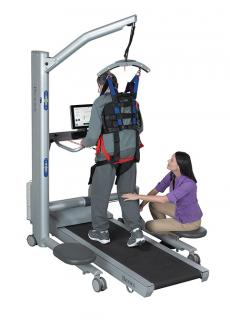
\includegraphics[height=3in]{gait_training.jpg} % first figure itself
%		\caption{Conventional gait rehabilitation. \cite{gaitrehabgantry}}\label{fig:gantry}
%	\end{subfigure}\hfill
%	\begin{subfigure}{0.45\textwidth}
%		\centering
%		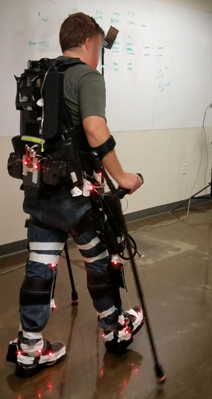
\includegraphics[height=3in]{subject.png}
%		\caption{EksoGT - powered exoskeleton}\label{fig:subject}
%	\end{subfigure}
%	\caption{Methods of gait rehabilitation}
%\end{figure}
%
%\begin{figure}
%	\centering
%	\begin{minipage}{0.45\textwidth}
%		\centering
%		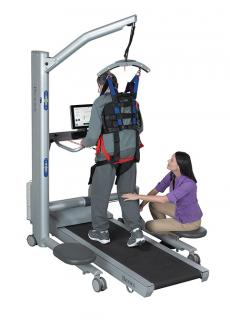
\includegraphics[height=3in]{gait_training.jpg} % first figure itself
%		\caption{Conventional gait rehabilitation. \cite{gaitrehabgantry}}\label{fig:gantry}
%	\end{minipage}\hfill
%	\begin{minipage}{0.45\textwidth}
%		\centering
%		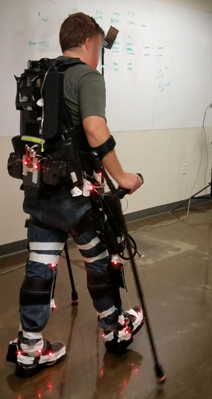
\includegraphics[height=3in]{subject.png}
%		\caption{EksoGT - powered exoskeleton}\label{fig:subject}
%	\end{minipage}
%\end{figure}
%
\begin{figure}
	\centering
	\subcaptionbox{Conventional gait rehabilitation. \label{fig:gantry}}[0.45\textwidth]{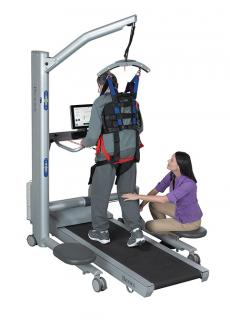
\includegraphics[height=3in]{gait_training.jpg}}%
	\hfill
	\subcaptionbox{EksoGT - powered exoskeleton \label{fig:subject}}[0.45\textwidth]{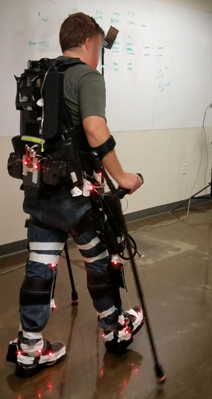
\includegraphics[height=3in]{subject.png}}%
	\caption{Methods of gait rehabilitation}
\end{figure}

\section{Motivation}
%
%\begin{figure}
%	\centering
%	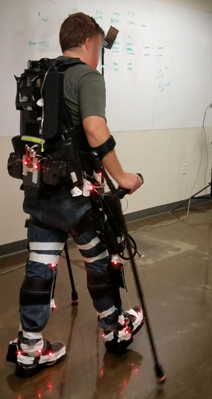
\includegraphics[width=0.15\linewidth]{subject.png}
%\end{figure}

Repeated walking practice has shown significant benefits in helping people with Spinal Cord Injury (SCI) achieve functional ambulation following initial injury \cite{lam2007systematic}. The US has a quarter-million existing cases of SCI with an additional 10,000 new cases annually \cite{nih}, and the cost of care per patient with SCIs exceeds half a million dollars~\cite{devivo2011costs}. Neural plasticity, i.e., the reorganization of the patient's intact neuronal pathways~\cite{curt2008recovery}, is one of the main mechanisms of recovery from SCIs. To take advantage of this neural plasticity, gait rehabilitation strategies involve repeatedly moving the patient's legs through prescribed walking trajectories. Conventionally, this process involves physiotherapists manually moving the patient's legs to track the desired trajectories (Fig.~\ref{fig:gantry} \cite{gaitrehabgantry}). %The main drawback of this approach is that the necessary joint trajectories may not be tracked accurately as the treatment progresses due to therapist exhaustion. 
As this approach requires physical intervention from therapists, the lack of therapist appointments, or the need to administer therapy virtually may affect its feasibility. Robotic exoskeletons have come into use for rehabilitation due to their ability to consistently track the desired trajectories, which may accelerate recovery~\cite{hidler2011role}. In this approach, the therapist acts in a supervisory role. Multiple exoskeletons, such as the Ekso GT \cite{brenner2016exploring} (Fig.~\ref{fig:subject}), Indego \cite{sup2008design}, and ReWalk \cite{rewalk}, have been cleared by the FDA for use in gait rehabilitation.

Exoskeleton usage increases the patient's level of autonomy, and fluent Human-Robot Interaction (HRI) is desired to maintain the safety and efficacy of the treatment. While an abstract notion, fluency in HRI can be roughly defined as the reliability with which a human and robot can predict each other's actions~\cite{hoffman2007cost}. In addition to device safety, increasing fluency would help the user locomote more naturally and reduce the effects of cognitive load \cite{bogen2018walk} on them caused by operating the device.

HRI fluency may be quantified by the inverse of the time it takes the human/robot pairing to complete desired tasks \cite{hoffman2019evaluating}. Fluency in HRI can be increased if the robot can anticipate the user's intent and assist accordingly. The overall goal of this work is to estimate user intent toward enabling increases in the fluency of lower-extremity exoskeletons. Intent itself is difficult to quantify, so a user's desired forward velocity is considered as an representation of their intent herein. Model-based and data-driven methods are considered to infer user intent by studying the effects of changes in velocity on gait patterns.

The rest of this chapter is organized as follows. Section~\ref{sec:overview} provides an overview of the various approaches to user intent estimation and their relevance to the work presented in this dissertation. Additionally, this section describes the role of HRI in user intent estimation. Section~\ref{sec:contribution} details the contributions of this dissertation.

\section{Overview: Intent estimation for fluency in HRI} \label{sec:overview}

A robot's ability to deliver timely assistance to the user is an important indicator of fluency. Anticipative intent estimation methods are necessary to reduce the delay in robot assistance delivery after the user has changed their intent, as the timing of the assistance is crucial for fluent HRI. Anticipative methods estimate intent changes before they are physically realized, in contrast to reactive methods that detect changes after realization. With anticipative inference, control actions necessary for assistance delivery may be decided in advance of when they need to be executed, and assistance may be delivered more precisely. Still, intent is an abstract concept, so it can be inferred in a variety of ways depending on how the estimation problem is posed. 

The user's desired gait speed is considered as the representation of their intent in this dissertation to enable quantification and estimation. A variety of physics-based models of legged locomotion have been used to describe human gaits, and the use of these for estimating gait speed is explored herein. However, the estimation problem is made challenging by the nature and severity of the exoskeleton users' injuries. Consequently, data-driven learning-based approaches have also been explored to address the aspects of user intent estimation that are difficult to model using physics-based models. These model-based and learning-based approaches are described in Section~\ref{sec:model_v_learning}. 

Aspects of human decision-making and intent realization are not well modeled using first principles, so it is difficult to use them to anticipate gait changes, and alternative approaches are required. Interactions between the user and robot may be informative of the user's intentions, and approaches to leveraging HRI are described in Section~\ref{sec:HRI}. The variability observed in walking patterns of people affects HRI and creates the need for user-specific estimation approaches. However, learning-based approaches may suffer from the lack of sufficient training to address the intra-subject and inter-subject variability. This personlization of estimation in the presence of data scarcity is described in Section~\ref{sec:personalization}.

\subsection{Model-based and learning-based approaches to estimation}\label{sec:model_v_learning}
Although humans are high degree-of-freedom systems, their gait patterns can often be accurately described by reduced-order models (Fig.~\ref{fig:abstraction}). Template and anchor models~\cite{full1999templates} are reduced-order models used to describe human walking. Template models emulate the salient characteristics of locomotion and abstract the complexities of neuro-muscular interaction. Anchor models are higher fidelity models based on human morphology that combine template models with human physiology. The additional complexities found in anchor models make estimation and control based on these models more computationally intensive, rendering them inappropriate for use in online processes such as intent detection. While detailed musculo-skeletal models offer subject-specific insight into walking, the omission of these complexities in template models make them more suited for general use across subjects. This generality and reduced order makes template models more suited for use in control and estimation problems for legged locomotion.

\begin{figure}
	\centering
	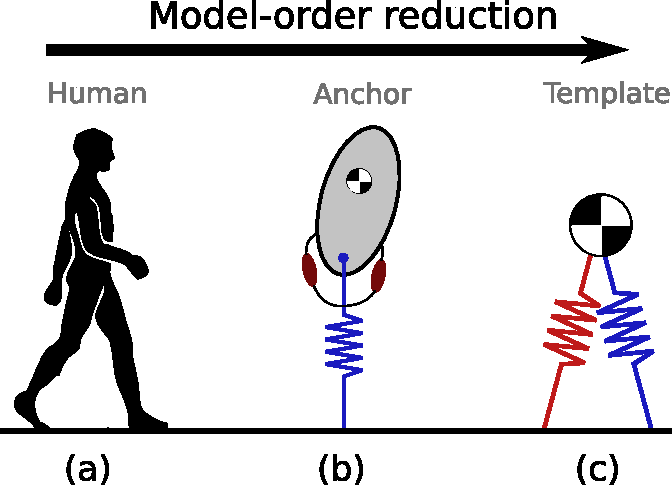
\includegraphics[width=0.55\linewidth]{abstraction.pdf}
	\caption[The model-order reduction of (a) a human; (b) an anchor model, a neuromuscular model where the hip is actuated using Hill-type muscle models, (c) a template model, Bipedal Spring-Loaded Inverted Pendulum model]{The model-order reduction of a human (a); (b) an anchor model, a neuromuscular model where the hip is actuated using Hill-type muscle models \cite{davoodi2019template}, (c) a template model, Bipedal Spring-Loaded Inverted Pendulum model \cite{geyer2006compliant}. }\label{fig:abstraction}
\end{figure}


Template models often use parameters such as center-of-mass (CoM) height, velocity, and leg stiffness to describe gait \cite{geyer2006compliant,liu2015dynamic,full1999templates,sharbafi2015fmch}. It may be possible to estimate an exoskeleton user's intended forward velocity by comparing measurements of these parameters with gaits simulated using models of locomotion with the general scheme illustrated in Fig.~\ref{fig:model_scheme}. For example, intent estimation in lower-extremity exoskeletons based on orbital energy \cite{chen2018dynamic} has been carried out using the Linear Inverted Pendulum (LIP) model, which is a simple model of legged locomotion.  Alternatively, data-driven estimation strategies \cite{ge2011neural, kalinowska2019data, joukov2017rhythmic} may be used to handle gait characteristics that are difficult to model using physics-based models.
%
%\begin{figure}
%	\centering
%	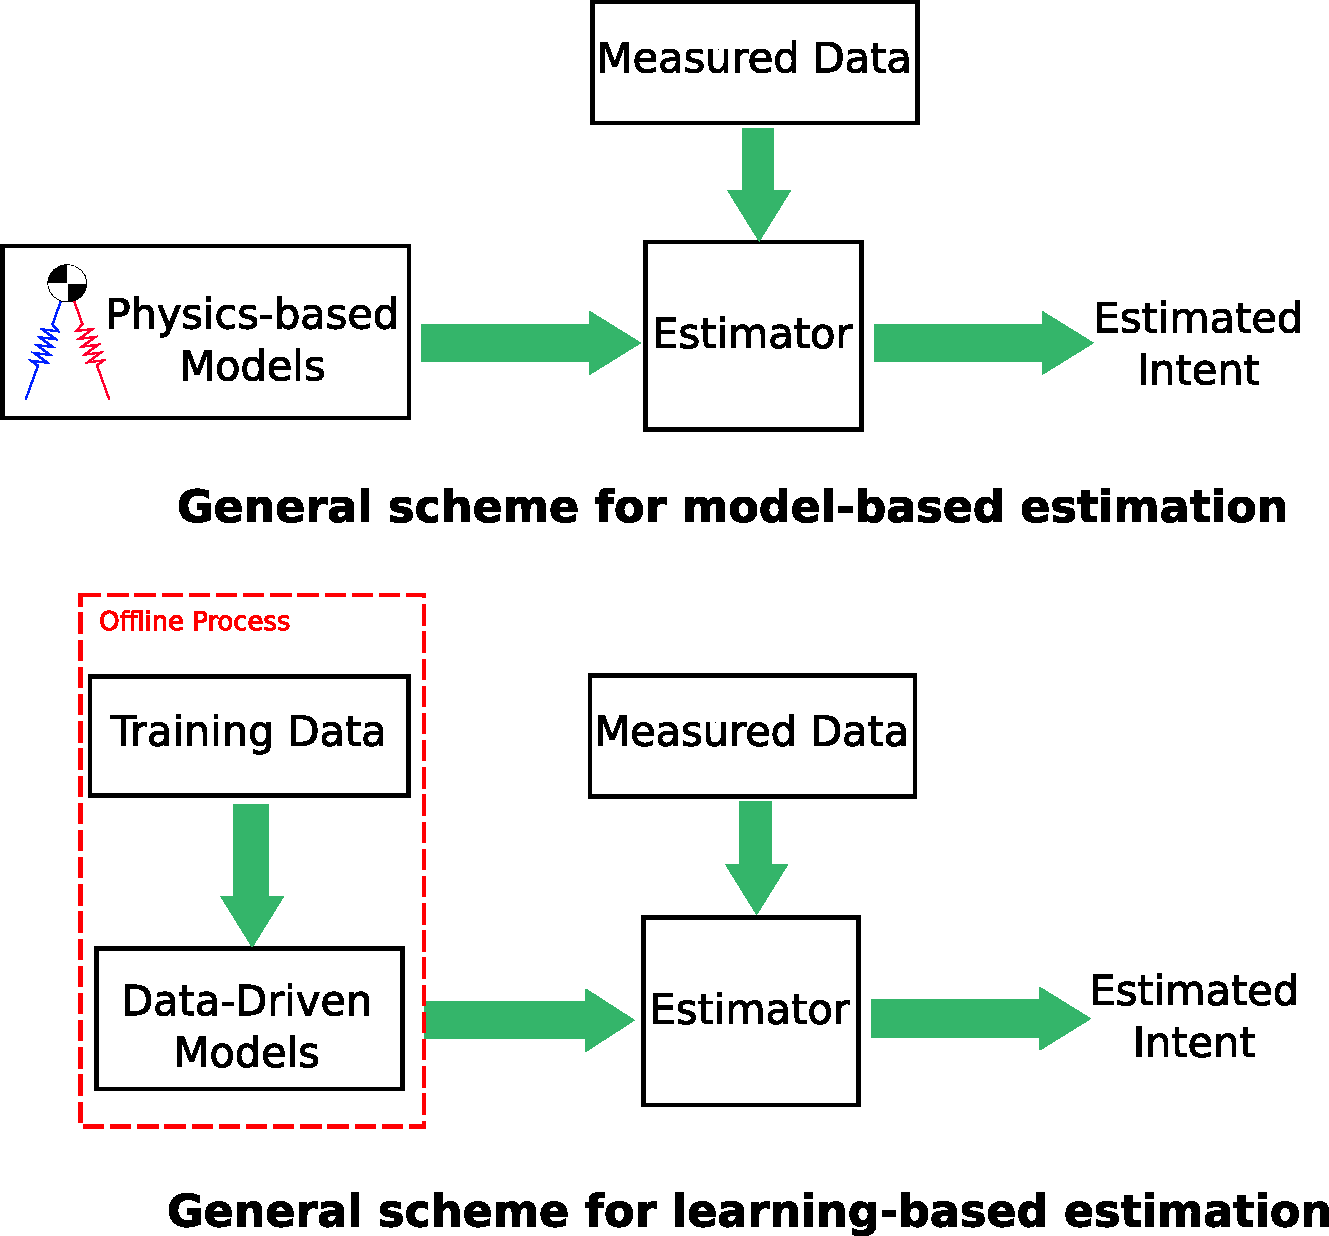
\includegraphics[width=0.6\linewidth]{schemes.pdf}
%	\caption{General overview of model-based and learning-based estimation}\label{fig:schemes}
%\end{figure}

Learning-based strategies use gait data to form relationships between sensor measurements and gait features such as foot placement and step frequency, and these relationships may then be used for estimating user intent, as illustrated in Fig~\ref{fig:learning_scheme}. Convolutional Neural Networks (CNNs) \cite{lee2020image}, decision trees \cite{moolchandani2021design}, and Linear Discriminant Analysis (LDA) \cite{young2013classifying}  have been more commonly used to infer user intent. These methods rely on sensors such as potentiometers and encoders onboard the assistive device \cite{young2013classifying}, electrogoniometers \cite{lee2020image}, and force plates \cite{moolchandani2021design} in addition to  electromyography (EMG) and Inertial Measurement Units (IMUs). A Gaussian Process (GP)-based Extended Kalman Filter has been used to estimate a user's gait phase during stance to control a powered prosthetic leg \cite{thatte2019robust}. These strategies require a large amount of training data, and this requirement may further increase when attempting to train user-independent models due to the inter-subject gait variability seen in human walking.

\begin{figure}
	\centering
	\setkeys{Gin}{width=\linewidth, keepaspectratio}
	\begin{subfigure}{\linewidth}
		\centering
		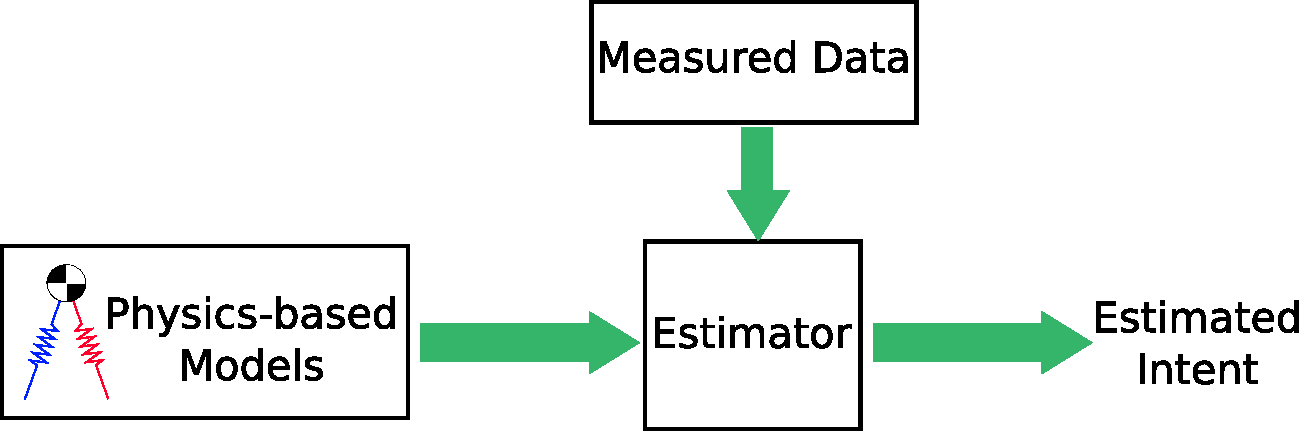
\includegraphics[width=0.6\linewidth]{model_scheme.pdf}
		\caption{General scheme for model-based estimation \label{fig:model_scheme}}
	\end{subfigure}
	\begin{subfigure}{\linewidth}
	\end{subfigure} 
	\begin{subfigure}{\linewidth}
		\centering
		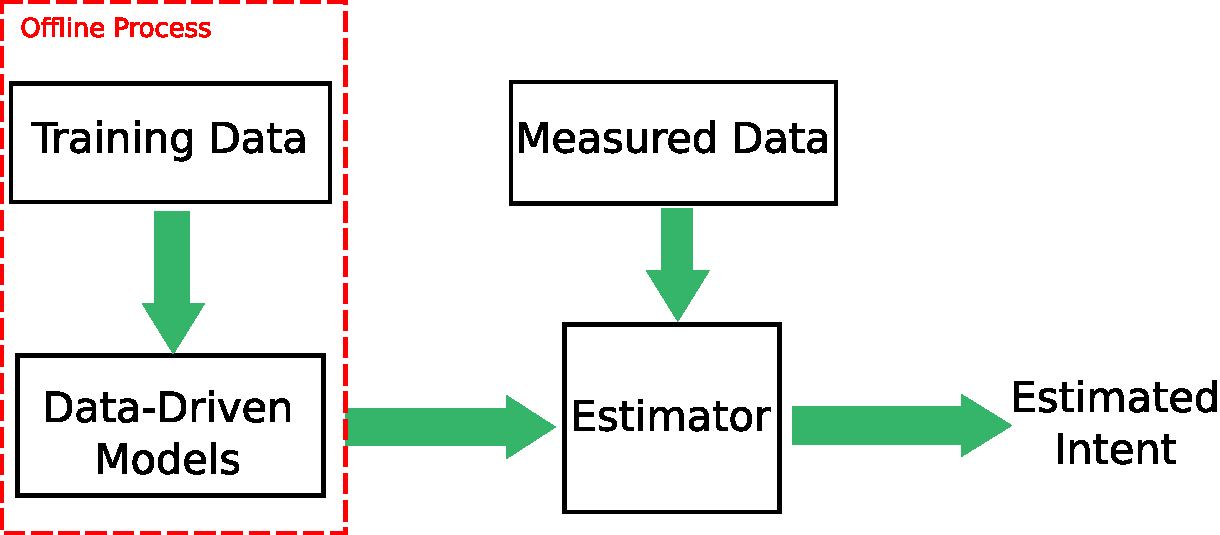
\includegraphics[width=0.6\linewidth]{learning_scheme.pdf}
		\caption{General scheme for learning-based estimation \label{fig:learning_scheme}}
	\end{subfigure}
	\vspace{-1em} 
	\caption{General overview of model-based and learning-based estimation \label{fig:schemes}}
	\vspace{-1em}
\end{figure}


\begin{figure}
	\centering
	\begin{overpic}[width=0.7\linewidth,percent]{intent_flow_chart.pdf}
		\put(14.5,23){\textcolor{NDgold}{\footnotesize \textbf{\cite{shen2013motion}}}}
		\put(31.5,3){\textcolor{NDgold}{\footnotesize \textbf{\cite{karulkarapplication,suzuki2007intention,brescianini2011ins}}}}
		\put(72,3){\textcolor{NDgold}{\footnotesize \textbf{\cite{Gambon20b,kalinowska2019data,thatte2019robust,sarac2013brain}}}}
	\end{overpic}
	\caption{Possible approaches to intent estimation. Approaches considered in this work have been indicated with green arrows.}\label{fig:flow}
	\vspace{-1em}
\end{figure} 

Different design decisions may be made when estimating user intent, as categorized in Fig.~\ref{fig:flow}. One approach is to infer intent posed as a discrete variable and infer it by comparing measurements of user activity to a database of predefined activities such as sitting, standing, steady-state walking, and the transitions between them \cite{shen2013motion}. Generating databases containing a wide range of such activities may be prohibitive due to challenges involved in human subject trials. Alternatively, intent may be treated as a continuous state to achieve finer control of the assistive device \cite{gambon2019characterizing, suzuki2007intention}. While there is some initial previous work regarding continuous speed estimation for prostheses \cite{best2021phase}, no such work is available regarding exoskeleton-assisted walking. Estimation strategies are often reactive and enable the inference of changes in a user's intent after they have been realized. Ideally, these strategies should be anticipative, as it would allow the robot to assist the user through the actions necessary to realize their desired changes. The actions a user takes to realize their desired changes often reflect in their interactions with the robot. Therefore, the patterns of a user's interaction with the robot may be informative of their desired collaborative actions.

\subsection{Leveraging HRI for intent estimation}\label{sec:HRI}

Estimation of user intent may be performed by leveraging the HRI in gait rehabilitation. One study used physical Human Robot Interaction (pHRI) to estimate the user intent in collaborative reaching motions  \cite{corteville2007human}. In it, the human was considered to be in control of the HRI, and measurements of the user's motion acquired using sensors onboard the robot were fit to a velocity profile to estimate the intended speed of the movement. 

Another approach to use pHRI for user intent estimation is to compare the user's efforts to the total effort necessary to accomplish the desired task \cite{pehlivan2015minimal}. Physical HRI is not limited only to interactions between the robot and the human. The human-robot system's interaction with the environment may also be considered pHRI and may be used to estimate user intent. For example, in a study by Brescianini \mbox{et al.,}~IMUs were mounted on crutches to estimate their orientation \cite{brescianini2011ins}. This configuration allowed the inference of user intent variables such as stride length, direction, and stair ascent/descent based on crutch placement. The reliance of many state-of-the-art approaches on additional external sensors like EMGs and force sensors may be challenging in practical applications. Some challenges are that EMG sensors need consistency in placement and may slip during usage due to perspiration~\mbox{\cite{tkach2010study,ison2014role}}, and sufficiently accurate wearable force sensors are not readily available~\cite{moolchandani2021design}. Therefore, relying on sensors onboard the exoskeleton may offer a more reliable option \cite{Gambon20b}. 

While pHRI may be used to infer an exoskeleton user's intent, the presence of injuries and their severity may limit the extent to which pHRI may be leveraged. HRI has been used to great effect in assisting healthy individuals walking in hip exoskeletons by modeling the impedance of the coupled human-robot system \cite{zhang2019admittance,nagarajan2016integral}. Hip torques generated by the user govern the assistance provided by the exoskeleton. However, it may be difficult to adapt these strategies to individuals with iSCIs due to significant lower-limb impairment. 

There are some available exoskeletons that are targeted toward individuals with iSCIs, and they use rudimentary methods to infer user intent. The HAL exoskeleton uses force sensors under the feet to detect weight transfer to initiate a step \cite{suzuki2007intention}, and the ReWalk system uses a combination of ground reaction force sensors and torso tilt~\cite{goffer2012locomotion}. While these intent detection strategies leverage basic pHRI, using additional gait variables to obtain information for intent estimation may provide additional insight into the user's desired motion. An exoskeleton's gait patterns may be analyzed to infer their intent using model- or learning-based strategies, proceeding to the third level of Fig.~\ref{fig:flow}. 

The work in this dissertation is targeted toward individuals with iSCIs who have limited mobility. Many of the state-of-the-art intent estimation strategies are reactive; however, an anticipative strategy may be better suited for this application as it would enable the exoskeleton to better react to a user's desire to change gait speed and assist accordingly. Additionally, many of these strategies are designed for use in prosthetic devices \cite{young2013classifying,young2015classification,massalin2017user,thatte2019robust}, and limited work for exoskeletons exists in literature \cite{medrano2022analysis}. Changes in gait speed correspond to changes in gait patterns that may be measured to help predict the user's intended walking speed. Gait patterns of people with \mbox{iSCIs} depend on the severity of the injury \cite{rota2011walk}. Therefore, subjects' interactions with the robot and the environment may show individualized trends making estimator personalization necessary for intent change estimation from gait patterns. 

\subsection{Personalizing intent estimation and addressing data scarcity}\label{sec:personalization}

Learning-based approaches for intent estimation often rely on large amounts of data to generate models of gait features \cite{lee2020image,moolchandani2021design}. Acquiring this data for an injured population is made increasingly difficult due to changes in gait patterns resulting from the severity of injuries \cite{sohn2018variability}. The difference in gait patterns across individuals makes the need for estimator personalization unavoidable. It is difficult to acquire adequate amounts of data to train models for estimation and deal with the gait variability resulting from spasticity due to iSCIs \cite{krawetz1996gait}. Data scarcity may be addressed by pooling training data from multiple subjects.

There is underlying commonality, across individuals, in changes to gait patterns relating to changes in gait velocity \cite{li1999coordination}. For example, changes in step length and frequency, pitch and roll motions of the torso, and joint trajectories all show qualitatively similar trends relating to changes in the desired gait velocity across individuals. This approach relies on user-independence of data that has been previously explored for uninjured individuals \cite{ibrahim2008gait, kilmartin2009optimising, wang2008accelerometry} and prosthesis users \cite{young2015classification}. However, considering user-independence of gait patterns for exoskeleton users with iSCIs is challenging due to the gait variability arising from the coupled dynamics of the human-robot system and spasticity arising from \mbox{iSCIs}. A large amount of training data is required to address this variability. The resulting data scarcity may be addressed by exploiting the commonality in gait patterns across individuals to personalize intent estimation by transforming easily accessible gait data from healthy individuals using a small amount of appropriately selected user-specific data.

\section{Contributions and organization}\label{sec:contribution}

Multiple robotic exoskeletons have been approved by the FDA for gait rehabilitation of individuals with iSCIs, yet the intent change estimation in these devices is reactive and limited to detecting when the user wants to initiate a new step of a predefined gait pattern. This limitation also prevents sudden velocity changes. As a result, these devices are generally seen in clinical settings, and their operation requires physiotherapist supervision. Anticipative user intent estimation in these devices may take these devices closer to being used unsupervised, toward increased usage and accelerated rehabilitation \cite{hidler2011role}. This dissertation makes contributions with an aim to advance the state of the art of intent estimation to be more anticipative of changes in the user's intent as represented through gait speed.

Chapter~\ref{chapter:bg_info} focuses on background information that forms the foundation of the contributions presented herein. This chapter discusses the basics of modeling human locomotion and gait periodicity using Poincar\'e maps. Additionally, the chapter explains the concept of state estimation with Kalman filters and describes two variations of the filter. Details of the exoskeleton trial data used to evaluate the estimators presented herein are also included in this chapter.

\begin{figure}
	\centering
	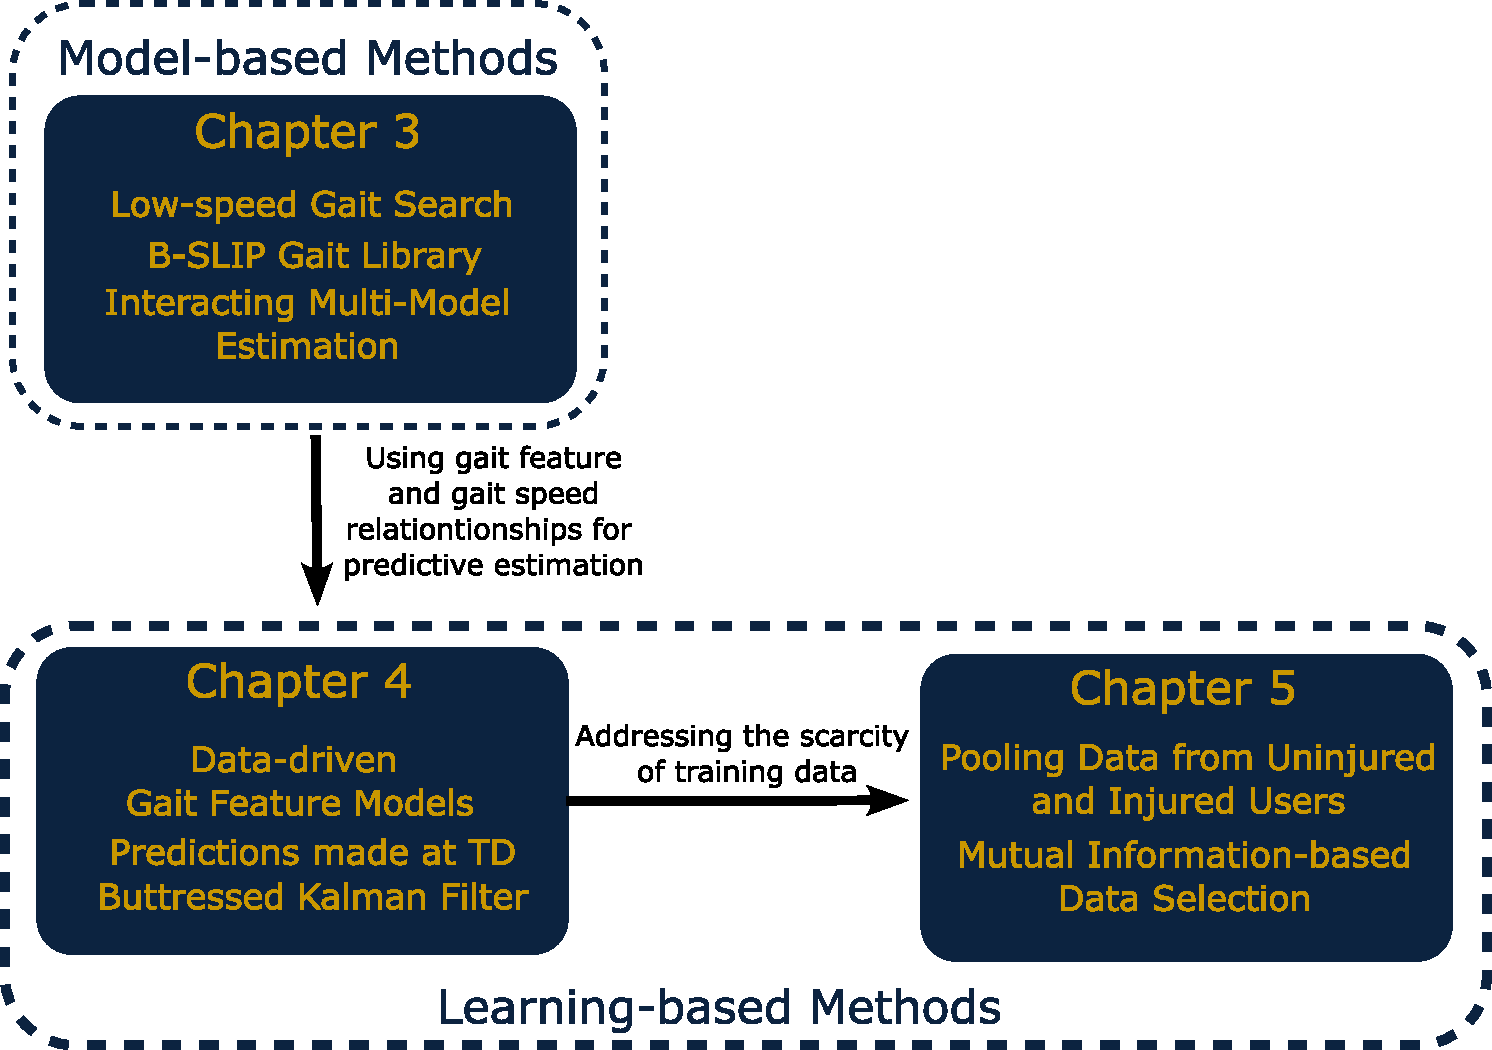
\includegraphics[width = 0.87\linewidth]{chapter_flowchart.pdf}
	\caption{Dissertation chapter overview \label{fig:chapter_flowchart}}
\end{figure}

As illustrated in Fig.~\ref{fig:chapter_flowchart}, the contributions presented in this dissertation span model-based and learning-based methods. The first contribution of the dissertation (Chapter~\ref{chapter:IMM}) studies the gait patterns seen during slow walking and establish an Interacting Multi-Model (IMM) estimation framework capable of handling hybrid dynamics seen in models of legged locomotion. Accurate state estimation is a foundational component for intuitive user intent detection in HRI, as it would deliver increased insight into user actions. Therefore, the IMM framework was used to estimate gait characteristics such as gait phase, by comparing simulated gaits of physics-based models of legged locomotion to measurements taken during walking trials with the exoskeleton. 

The work presented in Chapter~\ref{chapter:BKF} details a two-stage estimator, termed the Buttressed Kalman Filter (BKF), that anticipates changes in the exoskeleton user’s walking speed. This estimator was developed using the insights about walking in an exoskeleton, such as the changes in a user's gait patterns relating to gait speed, gained from the previous chapter. In contrast to many state-of-the-art intent estimators that are reactive, the presented framework anticipatively estimates a user's desired gait speed by analyzing how the user interacts with the robot and the environment to realize the desired change. This estimator was evaluated with walking trial data of individuals with and without iSCIs walking in an EksoGT exoskeleton, and the differences in the HRI of injured and uninjured users were also explored. For uninjured users, the estimator used measurements of step length to estimate the changes in a user's walking speed. For users with iSCIs, the estimator used measurements of step length and RMS hip motor currents to improve estimation accuracy.

Chapter~\ref{chapter:MP} builds on the estimator framework presented in Chapter~\ref{chapter:BKF}. The inter-subject variability in gait patterns observed across exoskeleton users motivated estimator personalization for anticipating speed changes. Estimator personalization was achieved while addressing training data scarcity by exploiting commonalities in gait patterns across users and augmenting data from healthy subjects with user-specific data from subjects with iSCIs. The work presented in this chapter explores the use mutual information between measurements of gait speed and gait features to incorporate data from multiple subjects to generate the models used in the estimator. Additionally, the effects of the the user's choice of assistive ambulatory device, a walker or crutches, on the personalized estimator are also explored. On average, estimator personalization resulted in increased success in estimating the subjects' desire to change speed, with changes detected before they were physically realized.
%Additionally, the work presented in this chapter also describes methods to discover user-specific relevance of gait features to gait speed and ensure estimator quality while personalizing gait speed estimation.

Chapter~\ref{chapter:conc} provides concluding remarks and introduces topics for future work that have emerged from the work presented in this dissertation.

%\begin{itemize}
%	%\item \textbf{Contribution 1: Model-based Approach to Estimate Gait Characteristics:} 
%	\item Accurate state estimation is a foundational component for intuitive user intent detection in HRI, as it would deliver increased insight into user actions. The first contribution was to establish a framework capable of handling hybrid dynamics to estimate gait characteristics such as gait phase, using simulated gaits of physics-based models of legged locomotion (Chapter~\ref{chapter:IMM}).
%	%\item \textbf{Contribution 2: Intent Change Estimation Based on Physical Interactions of an Exoskeleton User:} 
%	\item In contrast to many state-of-the-art intent estimators that are reactive, this objective is to develop an estimator that anticipates changes in the exoskeleton user’s intended gait velocity by analyzing how the user interacts with the robot and the environment to realize the desired change. This estimator was evaluated with walking trial data of	individuals with and without iSCIs walking in an EksoGT exoskeleton. The differences in the interactions of injured and uninjured users was explored (Chapter~\ref{chapter:BKF}).
%	%\item \textbf{Contribution 3: Personalization of Estimation in the Presence of Data Scarcity:}
%	\item The inter-subject gait variability observed across individuals motivated personalizing estimation of changes in intended gait velocity of exoskeleton users. One of the main hurdles in achieving the required personalization is the scarcity of user-specific training data due to difficulty in acquisition. Estimator personalization was achieved by exploiting commonalities in gait patterns across users and augmenting base data from healthy subjects with user-specific data from subjects with injuries (Chapter~\ref{chapter:MP}).
%\end{itemize}